So far I have demonstrated that it is possible to design a type system for most
of real-world C. In particular, such a type system supports resource management
in the presence of complex control flow, variable scoping and aliasing, and has
a conceptually simple extension to handle loose evaluation order.

One of the features I glossed over was the subtle and complex rules regarding
pointer manipulations, which cannot be ignored or simplified away in practice,
especially given \kl{CN}'s headline goal (\cref{sec:cn-intro}) to work
correctly above pre-existing C programs and observed behaviour.

The subtlety around observed behaviour for pointer manipulations stems from the
competing forces which shaped C.\sidenote{Inherited portability requirements,
proximity to hardware, and the desire for more aggressive optimisations.} As I
explained in \cref{sec:c-lang}, a completely concrete view of pointers would
invalidate fundamental optimisations we would like to perform on our code, but
a completely abstract view where pointers cannot alias each other is simply
incompatible with C's ability to take addresses of variables and compute with
pointers (incremet, calculate offsets, cast them to and from integers).

Whilst many aspects of C are specified using an elaboration, the representation
of pointers, and the choice of rules for manipulating them, are factored out
into a \emph{memory interface}. This interface is visible in
\cref{fig:effectful-core-grammar}: the memory operations $\mathit{memop}$ and
the memory $\mathit{actions}$; a \intro{memory object model}\sidenote{Named so
to distinguish it from a memory model in a concurrency setting.} is an
implementation of that interface.

Remember that C has a lot of different stakeholders, and so a memory model
which is acceptable to the standards committee needs to walk a fine line
between being concrete enough to enable as many low-level idioms as possible,
whilst being abstract enough to permit as many optimisations as possible. The
key concept which enables this is the idea of pointer \intro{provenance},
tracking where a pointer came from. With this, because C allows casting to and
from integers, the question naturally arises about whether this provenance
should be tracked via integers or not. Unfortunately, that is not the only
choice point involved in coming up with an acceptable memory object model;
\sidetextcite{memarian2022cerberus} documents and explains the trade-offs
between this and other choices.

Any set of choices must nagivate the tension between allowing
low-level idioms relied upon by existing code, allowing opportunities for
optimisations exhibited by existing compilers, and limiting the scope of both.
The cost of doing so (in a consistent manner\sidenote{None of the memory models
discussed are consistent with all observed behaviour, and it is not clear that
there is a consistent one which would be.}) is that the so far preferred (but
not yet officially adopted) memory object model,
\kl{PNVI-ae-udi},\sidenote{Provenance not tracked via integers, for addresses
which are exposed and provenances user-disambiguated. I will explain this imminently.} is a
complex minefield of \kl{UB} no human should be expected to navigate
unassisted.

\kl{PVNI-ae-udi} is complex enough that even implementing it in a C
verification tool is undesirable, especially because in that context, it is
reasonable to place a small extra burden of annotation on the user if it
simplifies verifying the code. This is the motivation behind the development of
\kl{VIP},\sidecite{lepigre2022vip} a memory model which is sound with respect
to PNVI-ae-udi,\sidenote{Quoting from the paper, ``every PNVI-ae-udi step can
be simulated by a VIP step, and that every step that raises
\kl[UB]{undefined behaviour} in PNVI-ae-udi also raises \kl[UB]{undefined
behaviour} in VIP.''} but simpler (it is fine to reject more programs, i.e.\
have more \kl{UB}).

\kl{VIP} as a memory model is \emph{simpler}, but it is not trivial. It is
defined operationally as a step relation between concrete (i.e.\ not symbolic)
heavily structured heaps, and the steps have complex premises.

In this part, I will detail the challenges and choices I faced in designing,
formalising and implementing \kl{CN-VIP}, the memory model of \kl{CN} as a scheme
within the formalised and implemented type systems.
\begin{itemize}
    \item \textbf{Expressiveness vs simplicity.} \kl{VIP} makes a particular
        choices about its representation of pointers and integers, and relatedly
        about the idioms it supports. I will explain it, and the other
        design around it, both simpler and more expressive. In particular,
        I will explain important and subtle complexities around round-trip casts,
        \cinline{memcpy} and \cinline{memcmp}, which are handled in
        \kl{VIP}/\kl{PNVI-*} test-suite, but not discussed.
    \item \textbf{Integration into \kl{Kernel CN}.} As I mentioned in
        \cref{sec:res-terms}, the novel structure for heaps abstracts away
        some aspects of its representation. I will explain how I adapted the
        static and dynamic semantics to use \kl{VIP}, and proved the new system
        sound with less repeated effort than typical.
    \item \textbf{Implementation in \kl{CN}.} I will explain how I incrementally
        developed, gated and deployed a complex change to memory model of \kl{CN}.
        By the time I had designed and formalised \kl{CN-VIP}, \kl{CN} had
        users, a tutorial, a test-suite and a continuous integration pipeline,
        so I had to be careful in adding support for \kl{VIP}, avoid difficult
        code merges and test updates.
    \item \textbf{Impact on annotations and performance.} Finally, I will explain
        how switching over to \kl{CN-VIP} (without round-trip casts) impacted
        the annotations and performance on existing \kl{CN} tests and tutorial
        examples.
\end{itemize}

\chapter{Memory object models, explained}\label{chap:mem-model-explained}

\margintoc%

From the perspective of \kl{Core} and \kl{ResCore}, the memory object model
(\cref{fig:mem-model-intf}) is simply a choice of representation of pointers,
and the interface specified in the memory operations $memop$, and memory
$\mathit{actions}$.\sidenote{Plus some extra primitives to detect races between
unsequenced expressions, which I will ignore.}

\begin{marginfigure}
    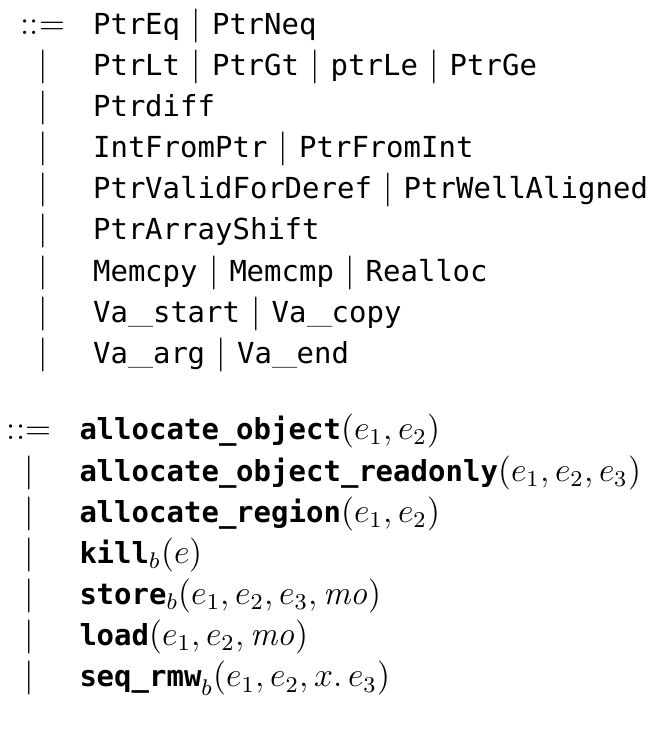
\includegraphics{figures/mem-model-intf}
    \caption{Memory model interface of \kl{Core}.}\label{fig:mem-model-intf}
\end{marginfigure}

The key concept which begins this brief overview of memory object models is
that of provenance. To optimise our code, compilers would like to assume that
not all pointers that a programmer can magically create (a) are valid, i.e.\
point to a live allocation (b) can alias any other live allocation in scope.

Let us revisit the example from \cref{fig:ptr-from-int}, reproduced in
\cref{fig:mem-model-ptr-from-int} for convenience. It shows a simple function
which takes an integer as an argument, assigns the number 5 to a local, and the
prints the value of that local, with some intervening pointer shenanigans.
Despite the fact that there is no data flowing between \cinline{k} and
\cinline{i}, the mere fact that the address of \cinline{j} was taken (and
``exposed'' via its assignment to an integer \cinline{k}) is enough to make the
compiler wary that the pointer \cinline{p} could alias \cinline{j} and thus
disable constant propagation.\sidenote{This example does have \kl{UB} though
because of (demonic) allocation address non-determinism.}

\begin{marginfigure}
    \centering
    \cfile{code/pointer_from_integer_1ie.c}
    \caption{Example pointer\_from\_integer\_1ie.c.}\label{fig:mem-model-ptr-from-int}
\end{marginfigure}

\clearpage%
\section{PNVI-ae-udi}

The rules justifying the above are set out in the \kl{PNVI-ae-udi} memory model,
upon which VIP is defined. Though the name is clunky and not euphonious, it is
descriptive as each part defines a particular choice to focus on.

\subsection{Provenance not tracked via integers}

For the purposes of defining the dynamic semantics of the memory object model,
each pointer can be thought of as an \emph{pair} of an address $a$ and an
provenance $\pi$. The address is simply what programmers might be familiar
with as `the pointer', which, unlike the provenance, may be inspected or
manipulated directly from the C program at runtime. From the perspective of
separation logic verification, the provenance can be thought of the ghost
part of a pointer, but it does play an integral part of the model of memory I
will outline next.

Allocation IDs (non-$@\mathsf{empty}$ provenances) are allocated fresh
globally\sidenote{PNVI-ae-udi does not support concurrency.} for every new
allocation, and thus guaranteed to be unique. An \intro{allocation history}
$\mathit{A}$ is a partial map indexed by allocation IDs, which tracks the size
of allocations, base address and whether or not they are live. The pointer
resulting from successfully creating a fresh allocation is a pair of base
address and the allocation ID\@. When an allocation is destroyed, the entry is
not removed, but merely updated to record the allocation as dead. The
allocation history includes other information too, which I will ignore because
it is not relevant to the key concepts.

The \kl{allocation history} merely tracks information about the allocation as a
whole, to track values of what resides in those allocations, \kl{PNVI-ae-udi}
also uses a memory $M$ as part of the abstract state. This is not just a map
from addresses to bytes, but triples of a (potentially empty) provenance and a
concrete 8-bit byte or $\mathsf{unspec}$ value for uninitialised or padding
bytes.\sidenote{There is an additional component, an optional \intro{pointer
    index} (an integer $j$ or $\mathsf{none}$) which stores which part of a
    pointer a byte came from. This is only relevant if either (a) pointer are
    not uniform, i.e.\ different pointers types can have different sizes or (b)
    provenance is tracked via integers (PVI) and bytes of those pointers have
    been overwritten.}\label{sn:ignore-ptr-index}

Reading from and writing to memory is done via the \coreinline{load} and
\coreinline{store} actions, at a specific C type, and these actions handle
structured \kl{Core} values, not sequences of bytes. Marshalling between the
two is handled via $\mathrm{repr}$ and $\mathrm{abst}$ functions. So for
example, a pointer $(a, @i)$ as a value is going to be stored as a sequence of
bytes in memory based on its address $a$, each byte with its provenance
$@i$.\sidenote{There is also an optional \kl{pointer index} for each byte's
position in the pointer, see note~\ref{sn:ignore-ptr-index}.}

One of the idioms existing code relies upon frequently is casting a pointer to
an integer and back again, and this \intro{round-trip} property is in fact
guaranteed by the ISO standard.\sidenote{§6.3.2.3\#5: An integer may be
    converted to any pointer type. Except as previously specified, the result
is implementation-defined, might not be correctly aligned, might not point to
an entity of the referenced type, and might be a trap representation.}. The
most obvious way to assign a provenance to a pointer created from casting an
integer is to simply track the provenance in the integer (PVI) when it was
casted \emph{from} a pointer earlier. However, the updates to the integer
operations to preserve their provenances would break the algebraic properties
of integers relied upon for optimisations by compilers.

Hence the reason for the first crucial design choice in PNVI-ae-udi: the
representation of integer values. As the name suggests, in contrast to PVI,
provenance is not tracked via integers. Casts of integers to pointers therefore
must pick some provenance: a first approximation is to say the result gets the
provenance of an allocation which is live at the time of the cast, whenever the
address is within its footprint.

\subsection{Ae: Considering only address-exposed allocations for round-trips}

Whilst the result of an integer-to-pointer cast getting the provenance of any
live allocation it happens to be contained in is a reasonable choice,
discussions with the standards committee, particularly the memory object model
study group, worried that this would forbid too many non-aliasing assumptions
(required for many optimisations to be applied validly).

A refinement of this approach is to limit the set of considered allocations to
not just the ones which are live, but also the ones which have their addresses
\intro{exposed} (-ae). The \kl{allocation history} would thus also track if an
allocation has been exposed or not, and the semantics of an integer-to-pointer
cast would then only examine those (\cref{fig:pnvi-ival-to-pval}).

\begin{figure*}
    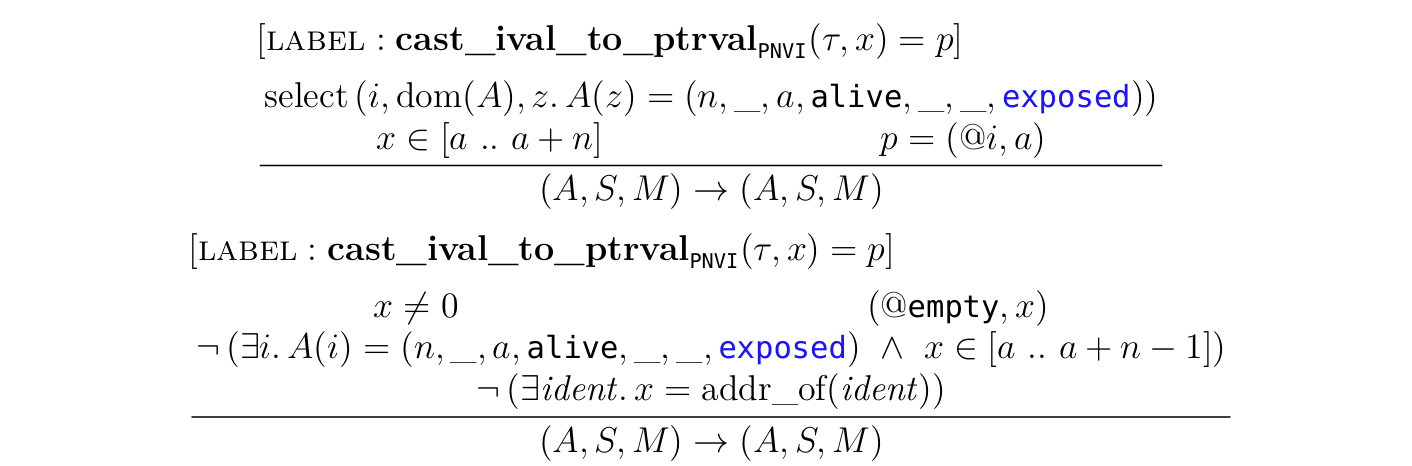
\includegraphics{figures/mem-model-pnvi-ival-to-pval}
    \caption{PNVI-* rules for casting an integer to a pointer. From
    \textcite{memarian2022cerberus}. The first rule should have $x \in [ a \;
        .. \; a + n - 1]$.}\label{fig:pnvi-ival-to-pval}
\end{figure*}

\begin{definition}[Exposed allocation]
An allocation is \emph{exposed} iff a pointer to anywhere within that
allocation
\begin{itemize}
    \item Is cast to an integer.
    \item Has its representation byte read (via a non-pointer lvalue).
    \item Is output via the format specifier \cinline|%p|.
\end{itemize}
\end{definition}

The `within that allocation' is key because one-past pointers (frequently used
to compare against the exclusive end of an allocation) which do not happen to
be that start of an adjacent object would then be assigned an empty provenance
$\mathsf{@empty}$. In turn, this would break the round-trip property required
of casts between pointers and integers for one-past pointers.

\subsection{Udi: disambiguating one-past pointers based on subsequent use}

Restoring round-trip casts for one-past pointers requires an additional
complication to the memory object model, \intro{symbolic} provenances. The
symbolic provenances are mapped to a set of either one or two allocation IDs
via an additional finite map $\mathit{S}$. Thus in the case where an integer
is cast to a one-past pointer on the boundary between two live allocations, its
provenance is assigned to be symbolic, containing both allocations' IDs
(\cref{fig:pnvi-ival-to-pval-symbolic}).

\begin{figure*}
    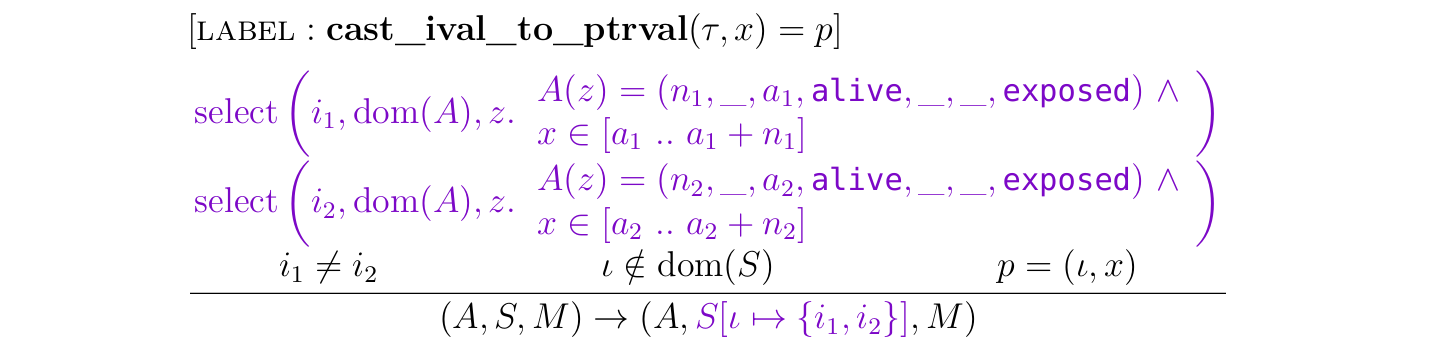
\includegraphics{figures/mem-model-pnvi-ival-to-pval-symbolic}
    \caption{PNVI-ae-udi rule for casting an integer to a pointer when
        the value is the address on the boundary between two live allocations.
        From \textcite{memarian2022cerberus}.}\label{fig:pnvi-ival-to-pval-symbolic}
\end{figure*}

Whilst useful for capturing many idioms and optimisations, the problem with these
symbolic provenances is that they complicate every other rule which requires
knowing the provenance of a pointer, usually to do some liveness and bounds checks.
Furthermore, these provenances can stay symbolic indefinitely, but if disambiguated
by what the user wrote (udi), must remain consistent from then onwards. The
most egregious example of this is the rule for subtracting pointers: there
are \emph{four} cases, \emph{three} of which stem from the existence of symbolic
provenances.
\begin{enumerate}
    \item \textbf{Neither pointer has symbolic provenance.} Both must be within
        bounds of the live allocation signified by their (equal) allocation
        IDs.
    \item \textbf{One pointer has symbolic provenance.} Both pointers must be
        within bounds of the live allocation signified by the concrete
        provenance, which must must be a member of symbolic one; the latter in
        turn is marked as disambiguated.
    \item \textbf{Both pointers have equal symbolic provenances.} Both must
        be within the bounds of either live allocations signified by the
        symbolic provenances, both of which remain ambiguous.
    \item \textbf{Both pointers have symbolic provenances with one in common.}
        Both must be within the bounds of the common live allocation, and
        both their symbolic provenances are marked as disambiguated.
\end{enumerate}

\section{VIP:\ Verified Integer Pointer Casts}

\kl{VIP}, by \sidetextcite{lepigre2022vip}, is a memory object model designed
to be a sound abstraction of PNVI-ae-udi. In particular, it relies on (the
acceptable trade-off of) requiring a small additional annotation burden to
simplify verification. Every \kl{UB}-free VIP program corresponds to a valid
PNVI-ae-udi program, and every \kl{UB} in \kl{PNVI-ae-udi} is also \kl{UB} in
\kl{VIP} (though \kl{VIP} itself may have more \kl{UB} than \kl{PNVI-ae-udi},
achieving its simplicity by increasing its restrictiveness).

\kl{VIP} achieves this by adding a single simplifying restriction on the
round-trip property: only integer values which were cast from pointers, with no
intervening operations, can be round-trip cast back to pointers. Any
intervening operation on that integer (including adding 0) will result in an
$\mathsf{@empty}$ provenance when cast to a pointer.

This restriction is sufficient to remove both \kl{exposure tracking} and
consequently \kl{symbolic provenances} and from the memory model of
\kl{PNVI-ae-udi}. This is because fundamentally VIP tracks exposure of specific
\emph{pointer values} rather than of whole allocations. Disallowing intervening
operations (even if the integer value remains within the bounds of the same
allocation) removes the need to do a search and bounds check of all live
allocation when casting back (I will discuss how \kl{VIP} recovers allocation
IDs in such cases soon). This also means that a boundary pointer is
disambiguated as soon as it is cast back, based on what it was cast from.

This restriction, particularly the `no intervening operation', forbids too
many desirable low-level idioms, such as pointer tagging.\sidenote{Programmers
store information in the lower or upper bits of pointers by exploiting platform
pointer alignment and addressable memory constraints respectively.} To
support these idioms, \kl{VIP} also provides a primitive, called
\cinline[breaklines]{void *copy_alloc_id(uintptr_t, void*)}, which lets a % chktex 36
programmer cast any integer to a pointer (with the appropriate checks).
This primitive is given both a direct semantics above the VIP abstract
state, and a translation into \kl{PNVI-ae-udi}.

The way that both of these are achieved is a very limited form of tracking
provenances via integers. Integer values in VIP model are represented by a
datatype with two constructors: $\mathit{Loc(@i, a)} \mid \mathit{Int(z \in
\mathbb{Z})}$. Casts from pointers $(@i, a)$ to integers just embed the pointer
into the $\mathit{Loc}$ constructor, and casts back to pointers just take the
value out (\cref{fig:vip-ival-to-pval}). If the integer value has any
intervening operations, only the integer parts (the address $a$ in
$\mathit{Loc}$, the payload $z$ in $\mathit{Int}$) are projected and used, any
provenance is forgotten (\cref{fig:vip-arith-binop}). If the integer has no
provenance, then \cinline{copy_alloc_id} can be used to annotate it with one
(\cref{fig:vip-copy-alloc-id}).

\begin{figure*}[tp]
    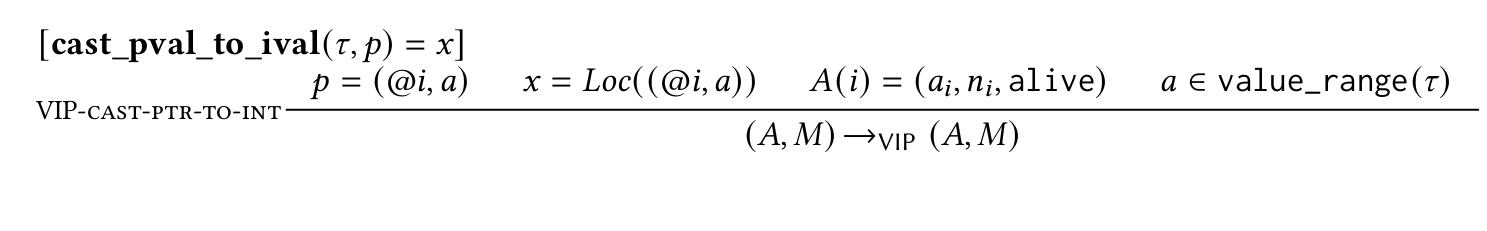
\includegraphics{figures/mem-model-vip-ival-to-pval}
    \caption{The \kl{VIP} rules to cast an integer into a pointer which
    preserves the round-trip property.}\label{fig:vip-ival-to-pval}
\end{figure*}

\begin{marginfigure}
    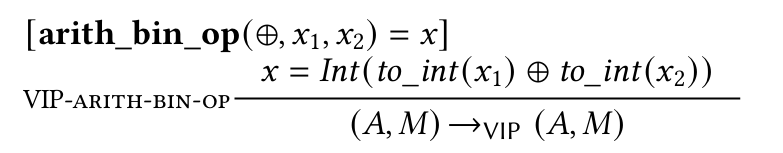
\includegraphics{figures/mem-model-vip-arith-binop}
    \caption{\kl{VIP} arithmetic operations on integers.}\label{fig:vip-arith-binop}
\end{marginfigure}

\begin{figure*}[tp]
    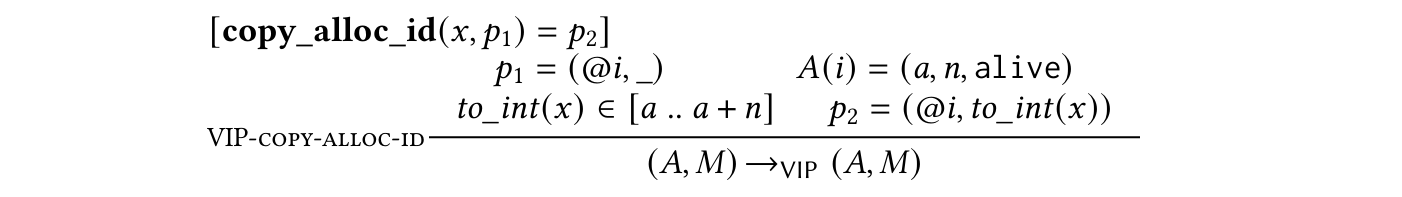
\includegraphics{figures/mem-model-vip-copy-alloc-id}
    \caption{\kl{VIP} \cinline{copy_alloc_id} primitive.}\label{fig:vip-copy-alloc-id}
\end{figure*}

The VIP \cinline{copy_alloc_id} primitive needs to be expressible in
PNVI-ae-udi for it to be a sound abstract, the way this is done is by
essentially implementing it as a C function
(\cref{fig:vip-copy-alloc-id-impl}). The implementation triggers two events in
\kl{PNVI-ae-udi}, the composition of which have the same effect as
\cinline{copy_alloc_id}: it ensures the allocation is \kl{exposed} by casting
it to an integer type, and then casts the integer to the pointer type. There
are some subtleties relating to the fact that the resulting provenance is
always concrete in \kl{VIP} but may be symbolic in \kl{PNVI-ae-udi}, but this
is not an issue because in well-defined programs, they differ only in
\emph{when} the disambiguation takes place (eagerly for \kl{VIP} and lazily for
\kl{PNVI-ae-udi}) rather than which way it disambiguates.

\begin{marginfigure}
    \cfile[breaklines,fontsize=\footnotesize]{code/copy_alloc_id.c}
    \caption{Implementation of \kl{VIP} \cinline{copy_alloc_id} primitive in C, to
        work above existing compilers, modelled via
        \kl{PNVI-ae-udi}.}\label{fig:vip-copy-alloc-id-impl}
\end{marginfigure}


\section{Design space}

Given this background, I will now consider some of the trade-offs involved
expressing different features of \kl{PNVI-ae-udi} and \kl{VIP} in \kl{CN}.

\subsection{Symbolic provenances}

Symbolic provenances initially seem like they should be easy to implement,
especially on top an SMT solver we use to do symbolic execution anyway. Whilst
the rules might be complicated, the potential advantage of not needing further
memory object model related annotations may be significant enough to be worth
it.

However, the symbolic nature of SMT problems turns out to not be helpful or
sufficient by itself to model symbolic provenances. The biggest reason why is
because of \intro{demonic allocation address non-determinism}. This is
orthogonal to \kl{PNVI-ae-udi} and \kl{VIP}, which are defined with respect to
a trace on a specific choice of addresses. It means that a program is deemed to
have \kl{UB} if there exists at least one choice of addresses for allocations
for which the memory object would signal \kl{UB}. In practise, this means that
the C program should not rely on objects being located at pre-determined
addresses or laid out with particular adjacencies, since both of those can be
changed with a different choice of addresses for allocations.

In a symbolic setting, this means an integer cast into an ambiguous one-past
pointer could belong to \emph{any} live allocation, not just one of two as in
the concrete address case.

Another serious problem is that the disambiguation of a provenance is a
\emph{relevant} fact: forgetting this would enable disambiguating the pointer
in inconsistent ways. This means that the disambiguation would need to be
tracked in the (linear) resource context, not the (intuitionistic) constraint
context.

So the choice is between: use annotations to thread pointer disambiguation in
pre- and postconditions, or or change the code to pass in a pointer with the
correct provenance to use with \cinline{copy_alloc_id}, forcing eager
disambiguation and sidestepping the associated implementation complexity. I
chose the latter.

\subsection{Exposure tracking}

Exposure tracking is another feature that \kl{PNVI-ae-udi} has but \kl{VIP}
does not. Remember that exposure tracking was devised to support round-trip
casts, but restrict the number of aliases which could be considered for the
results of those casts.

Exposure tracking has the distinct advantage over \kl{VIP} that round-trip
casts can happen (a) in the presence of intervening operations on the integer
value and (b) more importantly, \emph{without} a pointer to the specific
allocation we care about being available at runtime.

That being said, it is difficult to think of any idioms which require both of
these constraints to be true. One example is XOR linked-lists, where each node
stores the bitwise exclusive-or of the address of its previous and next
pointers, allowing a list to be traversed in forwards and reverse direction,
whilst saving the space for an additional pointer per node, and ``opinions
differ as to whether that idiom matters for modern
code''\sidecite{gustedt2021provenance}.

Unlike provenance disambiguation, exposure is an intuitionistic fact:
forgetting an exposure it would lead to fewer valid programs, but not
unsoundness. But still, this means that to be useful the trade-off here is
similar: use annotations to thread allocation exposure in pre- and
postconditions, or (if possible) change the code to pass in a pointer with the
correct provenance to use with \cinline{copy_alloc_id}. \kl{VIP} rules
already require tracking allocation liveness linearly, and so in principle,
adding exposure to that is not a very big change.

That being said, it is not clear to me how much this exposure tracking reflects
the analysis inside compilers, especially across functions. Address exposure
seems to be a syntactic over-approximation to pointer capture and escape
analyses.\sidenote{\url{https://jonasdevlieghere.com/post/escape-analysis-capture-tracking-in-llvm/}}
It seems unlikely to me that to me that if a call to a function exposed an
allocation, but did so without leaking any information about the exposed
address to the caller, that analyses in the caller would add that allocation to
the list of potential aliases resulting from an integer-to-pointer cast.

So whilst tracking allocation address exposure would be a reasonable choice,
especially given an important implementation advantage (which I will discuss
next), and would likely be sound with respect to \kl{PNVI-ae-udi}, I ultimately
decided that (a) it is not clear it is worth the additional complexity and (b)
it can be added later straightforwardly if the need arose.

\subsection{Provenance in integers and bytes}\label{subsec:prov-int-bytes}

It is a little ironic that after eschewing provenance via integers (\kl{PVI}),
that \kl{VIP} reinstates them albeit in a very limited form (i.e.\ not preserve
via integer operations to retain a simple theory of integers for optimisation).

From the view of a formalisation, an extra constructor or optional field on
each integer values does not make too much of a difference, since all the rules
handle this uniformly and sensibly. But, as I hinted at earlier, this comes
with a disadvantage for implementations above SMT solvers which, at first
glance, looks like it could be sidestepped by tracking exposure instead.

The concern with enriching the SMT representation of integers (currently
represented with plain bit vectors) is that it may lead to a slow down of
\emph{all} integer related problems handled by the SMT solver, and complicate
counter-examples for users. This presents us with four options.
\begin{itemize}
    \item \textbf{Drop support for round-trip casts.} Use only
        \cinline{copy_alloc_id} instead, at the cost of being able
        to verify fewer programs.
    \item \textbf{Add an extra constructor (or optional field) to the SMT
        representation of all integer types.} Support all \kl{VIP} verifiable
        programs, at the cost of the cost of complicating specification of
        and slowing verification for code which did not use this feature.
    \item \textbf{Restrict the ability to perform round-trip casts to new C
        types.} Require some modification to \kl{VIP} programs, but
        make any specification complication or performance penalty opt-in. This
        makes the user-visible memory object model more complex.\sidenote{For
            example, users opt-in with a
            \cinline[breaklines]{typedef uintptr_t rt_uintptr [[roundtrip]];}
            so the C program treats them identically, but \kl{CN} enforces a
            subtyping relation, so \cninline{rt_uintptr <:uintptr_t}.}\label{sn:optin-typedef-subtype}
    \item \textbf{Associate the provenance to \emph{a location} rather than a
        value, and track it in the resource system.} Such a resource would need
        to be duplicated, moved and destroyed in sync with the \emph{value} it
        is meant to be tracking via all memory actions.
\end{itemize}

There is another possibility, which we could entertain if we also allowed
exposure tracking:
\begin{itemize}
    \item \textbf{Recover provenance from ambient exposed allocations.} This
        would obviate the need to put allocation IDs in integer values at all.
\end{itemize}

If round-trip casts were the only issue related to provenance in integers, then
the situation would be relatively simple to handle. However, two of the
features of \kl{VIP} and \kl{PNVI-ae-udi} which does not get discussed very
much, but are quite important, is pointer bytes and
\cinline{memcpy}/\cinline{memcmp}.

In C, it is possible to take convert any pointer to an (\cinline{unsigned})
\cinline{char*} value and manipulate its byte representation. For example,
given a particular platform\sidenote{Endianness is an implementation-defined
property.} programmers can store information in the lower or upper bits of
pointers\sidenote{By exploiting platform pointer alignment and addressable
memory constraints respectively.} by writing to bytes of a pointer directly
\emph{without reading them first and thus exposing (parts of) their allocation
address}. So long as at least one byte remains of the original pointer, the
provenance is preserved.

A byte-level view of pointers also supports type-punning pointers via union
fields, since the representation bytes could be written at the pointer type,
and reinterpreted at another.

Relatedly, programmers can also \cinline{memcpy} pointers and use the copied
pointers in the destination \emph{with the provenance carried over}, or
\cinline{memcmp} pointers, though the semantics of this is to ignore
provenances and compare addresses only. A further complication arises from the
fact that if a programmer writes their own version of \cinline{memcpy}, then
that must also preserve provenance, and that calls to such code may validly be
replaced by a call to the library \cinline{memcpy} as a compiler
optimisation.\sidenote{\cinline{memcpy} does not expose allocations, but a
    user-defined one will, so justifying this optimisation is still an open
    question~\cite{gustedt2021provenance}. Additionally, the value of padding
    bits are unspecified (§6.2.6.2\#3).}

In both \kl{VIP} and \kl{PNVI-ae-udi}, all these use-cases are supported by
having the abstract bytes in the abstract memory $M$ store not just the
byte value (or \coreinline{unspecified}) but also a provenance. Pointer bytes
can be individually overwritten, but so long as one is untouched, the original
provenance can be recovered. Unions with a pointer field can be supported
similarly. Library \cinline{memcpy} simply copies over the abstract bytes to a
new location, and user-defined ones.

This leads to even more options.
\begin{itemize}
    \item \textbf{Drop support for byte-level provenance.} This would prevent
        manipulating pointer bytes, pointer type-punning in unions and
        user-defined \cinline{memcpy} from retaining provenance. It would
        also complicate the resource management required to have
        \cinline{memcpy} support copying provenances.\sidenote{Ideally,
            \cinline{memcpy} has a simple specification dealing with iterated
            ownerships of bytes, and leave handling structured values and
            resources (and the accompanying polymorphism) to other parts of the
            type system.}
    \item \textbf{Add an extra constructor (or optional field) to the SMT
        representation of characters}. Support all aforementioned idioms, at
        the cost of complicating specifications of and slowing verification for
        code which did not use this feature.
    \item \textbf{Restrict the ability to have provenance in bytes to a new C
        type.} Require some modification to \kl{VIP} programs, but make any
        performance penalty opt-in. This makes the user-visible memory object
        model more complex.\sidenote{See note~\ref{sn:optin-typedef-subtype}
        for a potential outline.}
    \item \textbf{Associate the provenance to \emph{a location} rather than a
        value, and track it in the resource system.} Such a resource would need
        to be duplicated, moved and destroyed in sync with the \emph{value} it
        is meant to be tracking via all memory actions.
\end{itemize}

There is another possibility, which we could entertain if we also allowed
exposure tracking:
\begin{itemize}
    \item \textbf{Prevent byte-level provenance features, \emph{unless} the
        allocation has already been exposed.} If the type system did
        track exposure, then the provenance could be recovered from ambient
        exposed allocations rather than from the bytes themselves.
\end{itemize}

The options for supporting round-trip casts are very similar to the options for
supporting byte-level provenance, even though on the surface, both features are
in principle, there to support very different low-level C idioms. This confluence
happens because:
\begin{itemize}
    \item In \kl{VIP} (unlike in \kl{PNVI-ae-udi}), round-trip casts are made
        possible by byte-level provenance (to preserve the $\mathit{Loc}$
        constructor through loads and stores).
    \item Both idioms seem to reflect a \emph{more general round-trip} property
        of casting (part of) a pointer to another representation and back.
    \item Both \cinline{char} and \cinline{uintptr_t} are \emph{integer} types in
        C, just of different widths. So it might be strange to a programmer if
        one supported round-trips but another did not.\sidenote{Fun fact: if
            its address is small enough, it is perfectly valid to cast a whole
            pointer into an \cinline{unsigned short} or \cinline{unsigned char}.}
\end{itemize}

In the face of these options, I first implemented \kl{VIP} \emph{without}
support for provenance in integers and bytes (in any form). This was
informative because it showed that the lack of provenance in bytes was much
more restrictive (on the \kl{VIP}/\kl{PNVI-ae-udi}) tests cases than the lack
of provenance in integers.

Considering this, and the options outlined above, I chose to restrict the
ability the features (supporting round-trip casts, and having provenance in
bytes) to different, new C types. Aside from making any complexity and
performance penalties opt-in, it also follows the convention set out in C++17
with the introduction \mintinline{cpp}{std::byte}, which is specifically
intended to be used to access byte representation of objects. For simplicity, I
chose to defer any implementation of subtyping resources automatically until
later.

\subsection{Non-deterministic pointer equality}\label{subsec:non-det-ptr-eq}

The official presentation of the \kl{VIP} memory model uses a strict variant of
the pointer-equality memory operation, which only looks at the addresses to
determine whether two pointers are considered equal.

Disappointingly, things are not quite so simple in actual C
(\cref{fig:nd-ptr-eq-example}). Because of provenance analysis, the compiler can
\emph{sometimes, but not always} detect when two pointers either side of an
equality test must have different provenances, and so optimise the result to be
false.

\begin{marginfigure}
    \cfile[breaklines]{code/provenance_equality_global_yx.c}
    \caption{An example C program which prints identical addresses but
        in some cases, a false result for pointer equality.}\label{fig:nd-ptr-eq-example}
\end{marginfigure}

Therefore, when the pointers either side of an \cinline{==} have equal
addresses but distinct provenances are distinct, the result will be
non-deterministic true or false (\cref{fig:nd-ptr-eq}). In practice, this will
only happen if either or both of the pointers are one-past, out-of-bounds as
the result of permissive array/member shift, or have an $@\mathsf{empty}$
provenance as the result of a cast from an integer.

\begin{figure*}
    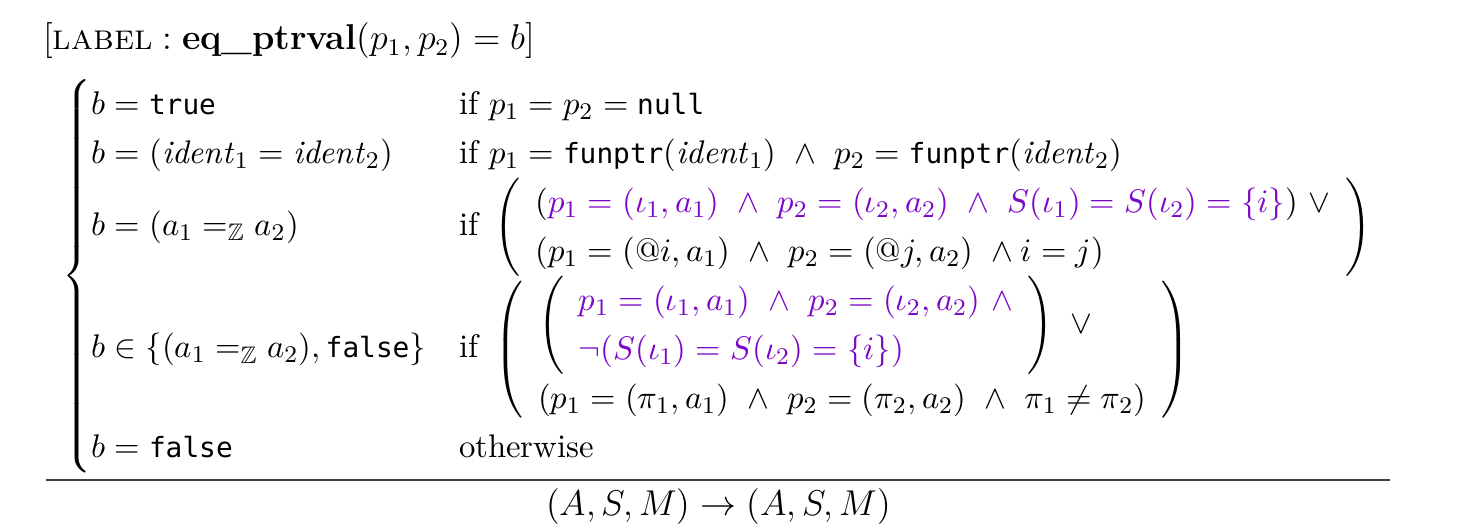
\includegraphics{figures/mem-model-pnvi-nd-ptr-eq}
    \caption{The \kl{PNVI-ae-udi} rule for pointer equality. When addresses
        are equal but provenances are distinct (captured by the fourth case),
        the result of \cinline{==} operator will be non-deterministically either
        true or false.}\label{fig:nd-ptr-eq}
\end{figure*}

This introduces a small syntactic inconsistency between the specification
language and C:\ in \kl{CN}'s specification language, \cninline{==} means
equality of pointers (address and provenance), but in C, \cinline{==} has
this strange non-deterministic behaviour. I sidestepped this issue by issuing a
warning whenever users write \cninline{==} in their specifications, pointing
them towards more informative (but verbose) named functions such as
\cninline{ptr_eq}, \cninline{addr_eq}, and \cninline{is_null}.

Unfortunately, adapting \kl{VIP} to handle the non-deterministic
pointer-equality rule is not straightforward. As it is defined in the paper and
appendix, they assume strict (address-only) pointer-equality rule for both
\kl{VIP} and \kl{PNVI-ae-udi}. This means they sidestep the issue I present
next.

Let us imagine we simply replace the strict (address-only) pointer equality
rule with the non-deterministic variant in both \kl{VIP} and \kl{PNVI-ae-udi}
at the same time. One aspect of soundness is that if \kl{PNVI-ae-udi} and
\kl{VIP} start in related states, then taking related steps will result in
either \kl{UB} in \kl{VIP}, or will end in related states, with related (equal)
return values. Now consider the example in \cref{fig:vip-non-det-ptr-eq-problem}.

\begin{marginfigure}
    \cfile[breaklines]{code/vip-non-det-ptr-eq-problem.c}
    \caption{Example code which exhibits non-deterministic behaviour under
        \kl{PNVI-ae-udi} (with non-det.\ pointer equality), but is always false
        under \kl{VIP} (with non-det.\ pointer equality).}\label{fig:vip-non-det-ptr-eq-problem}
\end{marginfigure}

\begin{itemize}
    \item In such a variant of \kl{PNVI-ae-udi} both pointers are one-past, and
        so have symbolic provenance, but the same address, and so the result is
        non-deterministic.
    \item In such a variant of \kl{VIP}, both pointers have $@\mathsf{empty}$
        provenance, so the equality test must return false.
    \item Both are valid steps, so in particular, the \kl{VIP} system does not demonstrate \kl{UB}.
    \item However, the return values cannot be related. The potential `true'
        branch for \kl{PNVI-ae-udi} could lead to \kl{UB} which would have
        incorrectly been classed as impossible in \kl{VIP}.
\end{itemize}

Both steps start in related states; the relation given in the proof of
soundness says that any provenance $\pi$ in \kl{PNVI-ae-udi} may be related
($\pi \approx_w @\mathsf{empty}$) to an empty one in \kl{VIP}. But if two
pointer both have $@\mathsf{empty}$ provenances in VIP, then we are free to
choose pointers with distinct provenances in \kl{PNVI-ae-udi}, to force the
pointer-equality operation to end up in the non-deterministic case. At this
point, the result values are no longer related by equality, and cannot be,
since the non-deterministic value can affect control flow and trigger \kl{UB}
in the path not taken by the \kl{VIP} variant.

The key insight is that the statement ``$@\mathsf{empty}$ provenances lead to
strictly more \kl{UB} than other provenances'', \emph{does not hold} in the
presence of the totally-defined, non-deterministic pointer-equality rule,
expressed in the proof by the relation $\pi \approx_w @\mathsf{empty}$. In
domain theoretic terms, if $@\mathsf{empty} \sqsubseteq \pi$ is supposed to
reflect the information ordering, the issue is that the pointer equality rule
is not monotonic with respect to this.

This presents us with the classic ``pick two of three'' situation:
\begin{itemize}
    \item \textbf{Drop $@\mathsf{empty}$ provenances.} This adds more \kl{UB}
        to CN's memory model, but it forbids the counter-example in
        \cref{fig:vip-non-det-ptr-eq-problem} and other soundness
        issues.\sidenote{Proof pending. Would have to redo above PNVI-ae-udi.}
        In practice, the change is small, primarily just forbidding the integer
        to pointer cast which is not a direct round-trip, requiring the
        programmer to use \cinline{copy_alloc_id} instead.
    \item \textbf{Drop totality for pointer equality.} An alternative approach
        would be to make the pointer equality test \kl{UB} if either argument
        has the $@\mathsf{empty}$ provenance. This would mean accepting a
        different interpretation/information ordering for empty provenances.
    \item \textbf{Drop non-determinism for pointer equality.} The existing
        \kl{VIP} system is sound with respect to \kl{PNVI-ae-udi} with strict
        (address-only) pointer equality, meaning no non-determinism.
\end{itemize}

\subsection{Allocation history}\label{subsec:alloc-history}

The allocation history in \kl{VIP} and \kl{PNVI-ae-udi} is mostly append-only
(new allocation are added, but old allocations are never removed) with the
exception that when an allocation is \coreinline{kill}ed, a boolean flag in its
entry (which is marked true when it is created) is set to false.

An allocation being live is important for some pointer operations, such as
relational ones, which require the operand pointers to be in bounds of the same
live allocation for the operation to not have \kl{UB}. However, for other
operations (such as member shifting), it must still satisfy a bounds check, but
whether or not an allocation is live is irrelevant. There is no operation which
requires knowing that an allocation is dead.

So bounds checks do not require live allocation, some operations require
live allocations but do not change that, and \coreinline{kill} requires
a live allocation but changes this.

As such, in \kl{CN}, I chose to represent the bounds check information as
\emph{constraints}, whereas I chose to represent liveness itself as an
\emph{allocation token} \cninline{Alloc}.

For the former, the type system and programmers need a way to refer to the
allocation history. It can be thought of as an implicit logical parameter
passed into and out of every function, and so I model it with an initially
unconstrained SMT variable. As \kl{CN} type-checks a \kl{ResCore} program, it
will learn constraints (either from creating new allocations, or from
postconditions of called functions, or derive them from allocation tokens in
the resource context) on the allocation history.

For the latter, though \cninline{Alloc} does take a pointer as an argument,
unlike \cninline{Block}, \cninline{Owned} and user-defined predicates, the
lookup in the resource context looks only at the allocation ID (the non-empty
provenance), not the address of the pointer.\sidenote{I need to update the
typing rules to reflect this.}

Unlike pointer disjointness facts based on \coreinline{Owned} and
\coreinline{Block}, I do not derive allocation or ID disjointness facts from
multiple allocation tokens, since there has been no visible need for it
yet.\sidenote{The only rule which needs to know whether to provenances are
\emph{not} equal is the non-deterministic case in the pointer equality rule,
and a relatively simple, if not slightly confusing annotation,
\cninline[breaklines]{ptr_eq(p,q) || !addr_eq(p,q)} can rule that% chktex 26 chktex 36
out.}\label{sn:ptr-eq-annotation} Dead allocations may perfectly well overlap
with live ones, though their allocation IDs will still be distinct, so tracking
all forms of disjointness accurately would add significant complexity for
little benefit.

\subsection{SMT representations}

One of the tricky aspects of adapting the memory object models to \kl{CN} is
that the models are defined over \emph{concrete} values and executions, whereas
\kl{CN} is fundamentally computing over \emph{symbolic} values.

Another is that adding extra variables (for default values in an infinite
domain) to an SMT problem is cheap (both to implement and to query) but can
affect usability, or worse, soundness if done incorrectly. Using algebraic
datatypes and adding an extra constructor takes more time, and may slow down
queries, but is necessary when those extra constructors need to be inspected.

\paragraph{Addresses.}%
The advantage of using symbolic values for addresses, is that this gives us
(demonic) allocation address non-determinism for free (whilst cheerfully
sacrificing the ability to say anything about the layout of local or global
variables, without the use of lemmas).

\paragraph{Provenances.}%
Should provenances be concrete? This depends on how they are used \textemdash{}
for querying whether two are equal; for querying whether two are distinct (only
for non-deterministic pointer equality); for the non-$@\mathsf{empty}$ ones
(allocation IDs), used as keys to get the associated base address and size from
the allocation history.

\paragraph{Empty provenance.}%
Empty provenances are intrinsically tied to pointer equality, since the rule
as given in \kl{PNVI-ae-udi} is not monotonic with respect to the implicit assumption
that $@\mathsf{empty} \sqsubseteq \pi$. Still, we can entertain how one might
proceed in each of the three situations.
\begin{itemize}
    \item \textbf{Drop $@\mathsf{empty}$ provenances.} This requires
        no representation of this construct.
    \item \textbf{Drop totality for pointer equality.}
        A single/global unconstrained variable, with explicit constraints that
        non-empty provenances are not equal to it, would work.
    \item \textbf{Drop non-determinism for pointer equality.}
        A single/global unconstrained variable would work. However, since with
        this option, all rules are monotonic with respect to $@\mathsf{empty}$
        provenances, i.e.\ any rule which uses an empty provenance will end up
        failing its bounds checks and thus signalling \kl{UB}, there is no need
        to add non-empty provenance constraints to the context.
\end{itemize}

\paragraph{Non-empty provenances (allocation IDs).}%
As for non-$@\mathsf{empty}$ provenances (allocation IDs), it is simpler to
leave them symbolic rather than try assign concrete values to them: two pointer
arguments to a function can validly have the same or different provenances, and
so it is best to leave the user to write constraints about the (in)equality of % chktex 36
relevant provenances.

\paragraph{Omitting function pointers.}%
With the representation of provenance and addresses fixed, the representation
of pointers I chose was guided by that given in \kl{VIP} and \kl{PNVI-ae-udi}:
a special constructor for the \cinline{NULL} pointer, or a pair of a
provenance and address. I omit support for function pointers
because (a) \kl{CN} does not calling functions via pointers (b) it would need
care to integrate in a way so as to not be cumbersome. For example,in defining
predicates which take pointer arguments, almost all the time a pointer will be
intended to be either \cinline{NULL} or pointing an object, so it would be sensible to
have a default which opts out of the function pointer case.\sidenote{A refinement
type system for the CN specification language?}

\paragraph{\cinline{NULL} pointer.}%
Though I do not know why \cinline{NULL} is not represented as
$(@\mathsf{empty}, 0)$ in the memory model,\sidenote{My conjecture is that it
    was a historical accident where PVI was developed first and in that model,
    $(@\mathsf{empty}, 0)$ represented an integer value, so a separate value
was used to represent \cinline{NULL} pointers.} I did observe a
small but useful reason to have it as a separate constructor during
implementation. With pointer equality in C (non-deterministic or otherwise),
the only information that the true branch of a pointer equality test gives the
programmer is that the addresses are equal; it says nothing about the
provenances. Conversely, with non-deterministic pointer equality, the false
branch does \emph{not} guarantee that the addresses are distinct: they could be
equal but have distinct provenances.

As I mentioned in \nameref{subsec:alloc-history}, to deduce \cinline{p} equals
\cinline{q} from testing \cinline{p == q}, a programmer needs the slightly
confusing annotation that \cninline{ptr_eq(p,q) || !addr_eq(p,q)}.% chktex 26 chktex 36
This constraint excludes the counter-intuitive (and non-deterministic) case of
the provenances being distinct but the addresses equal.\sidenote{Stated another
way, it can be seen as a promise that neither of the pointers are one-past
pointers, nor out-of-bounds as the result of a permissive array/member shift,
nor have an empty provenance as a result of a cast from an integer. A
sufficient (but not necessary) condition for this is that both pointers are
strictly within bounds of their allocations.} Whilst \kl{CN} aims to minimise
obvious annotations, this one seems difficult to avoid due the
inherited complexity of pointer equality tests, and the complexity with
tracking allocation and ID disjointness in the type system.

However, whilst programmers do check two pointers for equality often, they
check whether or not pointers are \cinline{NULL} far more. If \cinline{NULL} is
represented by $(@\mathsf{empty}, 0)$, then (in the presence of permissive
array/member offsets, since the other cases cannot apply) such checks would
need constraints too. A distinct \coreinline{null} constructor removes the need
for adding such constraints before every null-check.

\paragraph{Uninitalised memory and padding bytes.}%
To convert ownership of a struct into ownership of its representation bytes,
one needs to take into account the initialisation status of the struct and its
fields, and its padding bytes. Whilst I track the former with a structured SMT
value $.\mathit{init}$ in the formalisation, in \kl{CN}, the distinction is
more coarse with \cninline{Block} for uninitialised ownership (write-only) and
\cninline{Owned} for initialised (read and write).\sidenote{See
\nameref{sec:partial-init-structs} for a discussion.} The resulting ownership
needs to permit reading from bytes which are safe to read from (and constrain
them appropriately), but forbid or handle carefully bytes from uninitialised
fields or padding bytes. Ideally, it does so uniformly, so that the ownership
can be passed to \cinline{memcpy} or similar functions in one piece.

This raises thorny questions about the semantics of reads from uninitialised
memory and padding bytes; thorny because the \kl{ISO} standard is not clear and
there is no consensus de facto practice. Completely banning reads from them is
not ideal because we would like to permit byte-by-byte copying if possible. At
the same time, the rest of the \kl{CN} presently forbids reads from
uninitialised memory,\sidenote{Which is fair in a verification context.} and it
would be inconsistent to subvert this design choice via accessing byte
representations.

\kl{Cerberus} opts for an defined semantics for reads of uninitialised objects,
involving a notion of \intro{unspecified values}\sidenote{From 4.6.2 in
    \textcite{memarian2022cerberus}: \textit{``\ldots an abstract unspecified
        value which is propagated by arithmetic in a strict way, with the
        exception that operations that can have undefined behaviour are
        daemonic \ldots the unsigned addition operator over integer types has
        no undefined behaviour \ldots applying an unspecified value as right
operand of the division operator has undefined behaviour \ldots When the
controlling expression of a statement evaluates to an unspecified value, the
control-flow will non-deterministically behave''.}} which maps quite well to
the notion of unconstrained variables in SMT solvers. However, it is too
permissive with respect to the current \cninline{Block}/\cninline{Owned}
scheme, so just mapping \cninline{Block} values to unconstrained
\cninline{Owned} bytes of the same type would not work. Doing so would also,
when converting ownership of the bytes back into structured values, lose the
distinction between which parts were \cninline{Block}s and which
\cninline{Owned}s.

\paragraph{Memory bytes.}%
As I mentioned before, the issue of pointer bytes meant that I chose to have a
new C type for manipulating the byte-level representation of C objects. Not
only does this need to handle provenance in bytes
(\cref{subsec:prov-int-bytes}), but also uninitialised and padding bytes as
mentioned above. As a result, I chose to represent the \intro{memory bytes} as
a datatype with two constructors: one for $\mathsf{unspec}$, one for a pair of
a 8-bit vector and an optional allocation ID (for writing and recovering
pointer provenance). The representation of \cninline{Block}s and padding bytes
are mapped to \cninline{unspec} values, the representation of \cninline{Owned}
values I map to their appropriate byte (depending on
index)\sidenote{\kl{Cerberus} does not currently support switching on
endianness, so I match its default big-endianness, which is also suitable for
verifying \kl{pKVM} on Arm}, and an allocation ID if it is part of a pointer.

\paragraph{Permissive array and member offsets}%
In \kl{VIP} and \kl{PNVI-ae-udi}, array and member offsets are only defined on
pointers with a provenance and permissive member shifts on a \cinline{NULL}
pointer result in pointers with an $@\mathsf{empty}$ provenance, and the
\cinline{offsetof} value in the address. However, when encoding these
operations in SMT problems, such offsetting needs to be total, defined on all
values, with the understanding that the type system should only symbolically
evaluate offsets on a pointer it can prove has a provenance. With an empty
provenance, the encoding is obvious, but in its absence, I fall back to the
standard idiom of using an unconstrained variable as a default value.

\subsection{Summary}

\begin{itemize}
    \item \textbf{All pointers on a platform are the same size.} This
        allows me to drop the pointer index component of the abstract bytes
        from the abstract memory (see note~\ref{sn:ignore-ptr-index}).
    \item \textbf{All provenances must be disambiguated immediately.} This
        requires using \cinline{copy_alloc_id}, but saves tracking
        disambiguation in the resource system (and sidesteps wondering what
        adjacent addresses look like in a symbolic evaluation setting).
    \item \textbf{Allocation address exposure is not tracked.} This prevents
        verifying code like XOR-lists, and complicates support for round-trip
        casts and limits options for byte-level provenance. If needed,
        implementing such tracking should be a straightforward extension in the
        future.
    \item \textbf{Initially, no support for provenances in integers or bytes
        (or a resource polymorphic \cinline{memcpy}).}
        This prevents a substantial amount of the \kl{VIP}/\kl{PNVI-ae-udi}
        test-suite from passing without additional annotations.
    \item \textbf{Later, support provenance in integers and bytes via new C
        types.} This makes their associated complexity and any performance
        penalties opt-in.
    \item \textbf{$@\mathsf{empty}$ provenances eliminated.} This enables
        soundly supporting total and non-deterministic pointer equality.
    \item \textbf{Allocation history tracked in constraints.} This makes
        bounds checks easy to state and check.
    \item \textbf{Allocation liveness (and disjointness) tracked in
        resources.} This leverages the existing resource context set up
        to manage allocations correctly and check if pointers are live.
    \item \textbf{Allocation and ID disjointness is not inferred.} Tracking
        this accurately would be complicated, and the benefit (of reducing
        annotations required for testing pointer equality) would be limited.
    \item \textbf{Use extra constructors for \cinline{NULL} and
        \coreinline{unspec}, and variables everywhere else.} This means using
        variables for addresses and allocation IDs and unconstrained ones as
        default values in morally partial operations.
\end{itemize}

\begin{figure}[h]
    \centering
    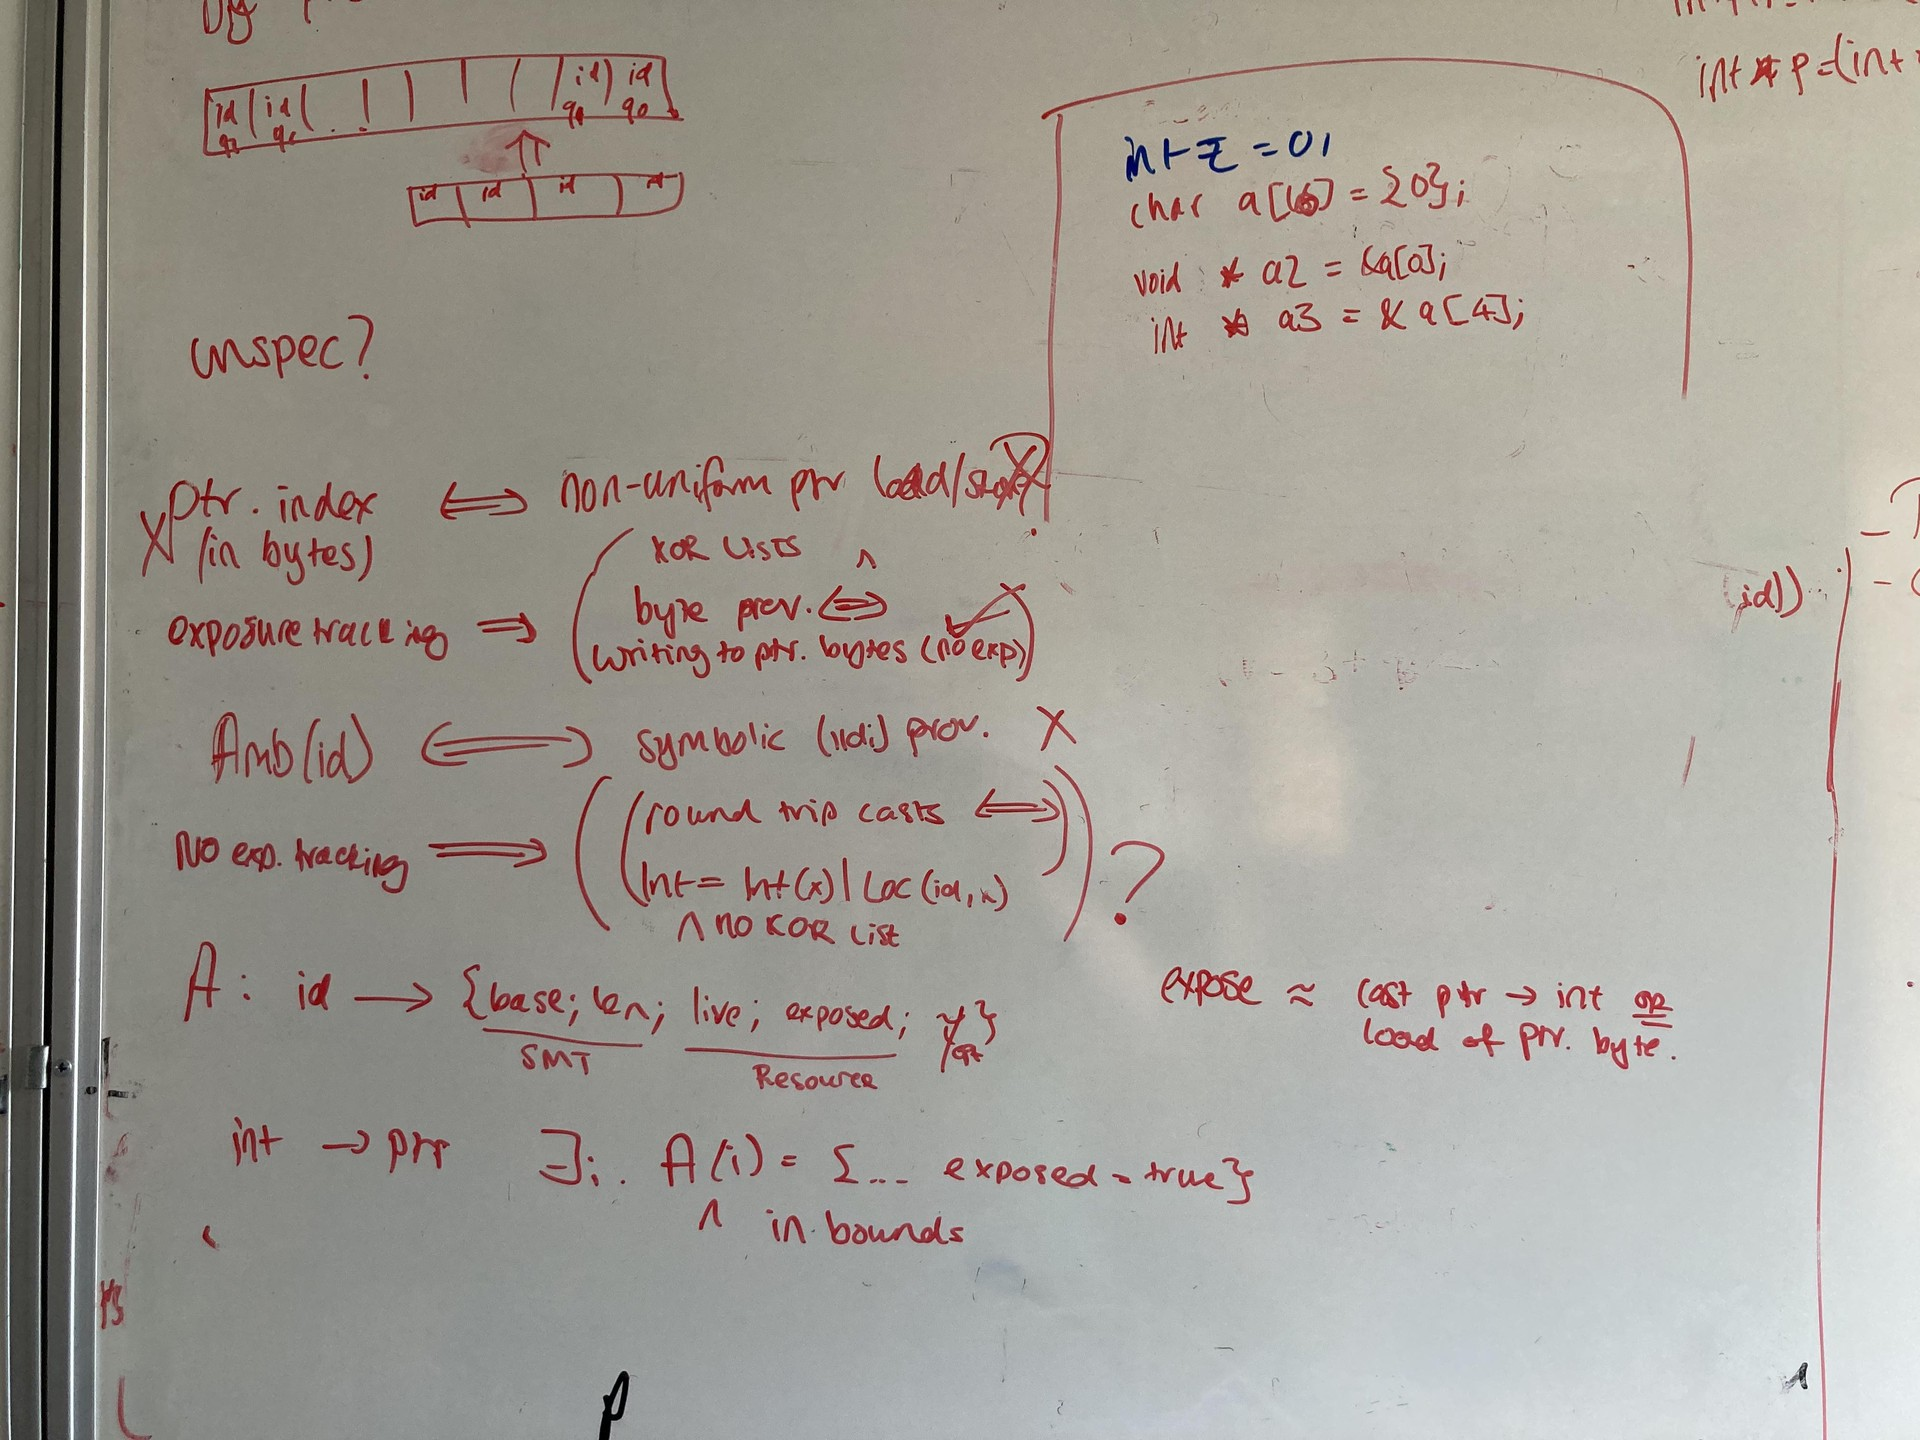
\includegraphics[width=\textwidth]{../misc/type-system-options.jpg}
\end{figure}
